%% LaTeX Beamer presentation template (requires beamer package)
%% see http://latex-beamer.sourceforge.net/
%% idea contributed by H. Turgut Uyar
%% template based on a template by Till Tantau
%% this template is still evolving - it might differ in future releases!

\documentclass[mathserif,trans]{beamer}
% [trans] no transitions
% [handout] handouts 



\mode<presentation>
{
 \usetheme{Warsaw}
 \useoutertheme[subsection=false]{smoothbars} %remove toc at begin of slide
\setbeamertemplate{items}[circle]
\setbeamertemplate{headline}[smoothbars theme]
\setbeamertemplate{sections/subsections in toc}[circle]
% \setbeamertemplate{mini frames}[box] % shows small rectangles as mini frames.
% \useinnertheme[shadow=true]{rounded}
% \setbeamertemplate{footline}[page number]{}
\setbeamertemplate{navigation symbols}{} %deletes navigation
\setbeameroption{hide notes}

% \setbeamercovered{transparent} %for transparency in items
}

\mode<handout>{
	\usetheme{default}
	\usepackage{pgfpages}
  
%   \setbeamercolor{background canvas}{bg=black!5}
  \pgfpagesuselayout{4 on 1}[border shrink=2.5mm]
}

\usepackage[english]{babel}
\usepackage[utf8]{inputenc}

% font definitions, try \usepackage{ae} instead of the following
% three lines if you don't like this look
\usepackage{mathptmx}
\usepackage[scaled=.90]{helvet}
\usepackage{courier}


%mktexpk --mfmode ljfour --bdpi 3600 --mag 1+0/3600 --dpi 3600 ubuntu

\usepackage[T1]{fontenc}
% \makeatletter
% \newif\if@restonecol
% \makeatother
% \let\algorithm\relax
% \let\endalgorithm\relax
\usepackage{algorithm2e}
\usepackage{pstricks}
\usepackage{pstricks-add}
% \usepackage{framed}
\usepackage{multirow}




% \font\ttfubuntu fonts/ubuntu at11pt
%FONTS \usepackage
% serif
% euler
% newcent
% avant
% helvet
% palatino
% bookman
% mathtime
% pifont
% chancery
% mathptm
% utopia
% charter
% mathptmx



\title{Integrity constraints in Cloud Databases}

%\subtitle{}

% - Use the \inst{?} command only if the authors have different
%   affiliation.
%\author{F.~Author\inst{1} \and S.~Another\inst{2}}
\author[\insertframenumber/\inserttotalframenumber\hspace{7em} Harsha
Raja]{Harsha Raja}

% - Use the \inst command only if there are several affiliations.
% - Keep it simple, no one is interested in your street address.
\institute[Victoria University of Wellington]
{
Victoria University of Wellington\\
Wellington, New Zealand\\
}

\date[IEEE-NZ]{IEEE - New Zealand 2011}


% This is only inserted into the PDF information catalog. Can be left
% out.
\subject{IEEE'11}



% If you have a file called "university-logo-filename.xxx", where xxx
% is a graphic format that can be processed by latex or pdflatex,
% resp., then you can add a logo as follows:

\pgfdeclareimage[height=0.5cm]{university-logo}{VUWlogo.eps}
\logo{\pgfuseimage{university-logo}}



% Delete this, if you do not want the table of contents to pop up at
% the beginning of each subsection:
% \AtBeginSubsection[]
% {
% \begin{frame}<beamer>
% \frametitle{Outline}
% \tableofcontents[currentsection,currentsubsection]
% \end{frame}
% }

% If you wish to uncover everything in a step-wise fashion, uncomment
% the following command:

%\beamerdefaultoverlayspecification{<+->}

\begin{document}

\begin{frame}
\titlepage
\end{frame}

\begin{frame}
\frametitle{Outline}
% \begin{block}{}
\tableofcontents[pausesections]
% \end{block}
% You might wish to add the option [pausesections]
\end{frame}


\section{Cloud Databases}
	\subsection{Fundamentals}
	
	\begin{frame}
		\frametitle{Cloud Databases}
		
		\begin{block}{Fundamentals}
			\begin{itemize}
			  \item What is?
			  \item How it became
			  \item Advantages
			  \item Importance
			\end{itemize}
		\end{block}
		
	\end{frame}
	
	
	\subsection{Challenges}
	
	\begin{frame}
		\frametitle{Challenges in Cloud Databases}
		
		\begin{block}{}
			\begin{itemize}
			  \item Replication
			  \item Updating data
			  \item Absence of Referential Integrity
			\end{itemize}
		\end{block}
		
	\end{frame}
	
	
% \section{Key-Value Databases}
	
	\subsection{Relational Databases}
	
	\begin{frame}
		\frametitle{Key-Value Databases}
		
		\begin{columns}
		
		\column{.5\textwidth}
		\begin{block}{Relational Databases}
			Present example
		\end{block}
		
		\column{.5\textwidth}
		\begin{block}{Key-Value Databases}
			Present example
		\end{block}
		
		\end{columns}
		
		
	\end{frame}
	
\section{Problem and Solutions}
	\subsection{Problem}
	\begin{frame}
		\frametitle{Problem in Cloud Databases}
		
		
		\begin{columns}
		
		\column{.5\textwidth}		
		\begin{block}{}
			Empty block
		\end{block}
		\column{.5\textwidth}
		\begin{block}{}
		
		\end{block}
		
		\end{columns}
	\end{frame}

\subsection{Solutions}
	
	\begin{frame}
		\frametitle{Solutions}
		\begin{block}{}
			\begin{enumerate}
			  \item Idea \# 1
			  \item Idea \# 2
			  \item Idea \# 3
			\end{enumerate}
		\end{block}
	\end{frame}
	




% \section{Introduction}
% \subsection*{Motivation}
% 
% \begin{frame}
% \frametitle{Introduction}
% \note{Not good way to start}
% \begin{block}{}
% \vspace{10pt}
% \begin{itemize}[<+->]
%   \setlength{\itemsep}{8pt}
% 	%there are many works using Asynchronous PSO
% 	\item Particle Swarm Optimization (PSO) is implicitly synchronous
%   \item Asynchronous PSO (APSO) by Carlisle and
%   Dozier (2001)
%   \begin{itemize}[<+->]
%     \setlength{\itemsep}{4pt}
%   	\item Comparison of APSO and SPSO on five benchmark functions
%   	\item Analysis based on descriptive statistics
%   	\item Conclusions: APSO is generally faster and (hence) less
%   	costly (iteration-wise)
%   	\item Cited more than 300 times, 60+ contained the word
%   	\alert{asynchronous} (Google Scholar).
%   \end{itemize} 
%   \item Statistical significance tests?
% \end{itemize}
% \vspace{10pt}
% \end{block}
% 
% \end{frame}
% 
% \subsection*{Objectives}
% \begin{frame}
% \frametitle{Objectives}
% \begin{block}{General objective}
% \centering
% Do statistical tests support that APSO is actually \textbf{\emph{better}} than
% SPSO?
% \end{block}
% \pause\begin{block}{Specific objectives}
% 	\begin{enumerate}[<+->]
% 	  \item Compare SPSO and APSO in ten benchmark functions
% 	  \item Perform statistical significance tests on the results
% 	  \item Assess the effect of different social network structures
% 	\end{enumerate}
% 	\vspace{0pt}
% \end{block}
% 
% \end{frame}
% 
% 
% 
% 
% 
% \section{Background}
% \subsection{Particle Swarm Optimization (PSO)}
% 
% \begin{frame}
% \frametitle{Particle Swarm Optimization (PSO)}
% \framesubtitle{}
% \begin{columns}
% \column{.5\textwidth}
% \begin{block}{Fundamentals}<1->
% \begin{itemize}
%   \item<2-> Population of particles
%   \item<3-> Share information
%   \item<4-> Move towards the best solutions found so far
%   \item<5-> Adjust their velocity according to experience
% \end{itemize}
% \end{block}
% 
% 
% \column{.5\textwidth}
% \begin{example}<1->
% {
% \centering
% \newcommand{\fwidth}{0.3\textwidth}
% \begin{figure}
% \setlength\fboxsep{0pt}
% \setlength\fboxrule{0.75pt}
% \begin{psmatrix}[mnode=R, colsep=0.2,rowsep=0.2]
% 	\onslide<1->\fbox{\includegraphics[width=\fwidth]{./figures/sphere-0.eps}} &
% 	\onslide<2->\fbox{\includegraphics[width=\fwidth]{./figures/sphere-1.eps}} &
% 	\onslide<4->\fbox{\includegraphics[width=\fwidth]{./figures/sphere-2.eps}}\\
% 	\onslide<5->\fbox{\includegraphics[width=\fwidth]{./figures/sphere-3.eps}} & 
% 	\onslide<6->\fbox{\includegraphics[width=\fwidth]{./figures/sphere-4.eps}} &
% 	\onslide<6->\fbox{\includegraphics[width=\fwidth]{./figures/sphere-5.eps}}
% \end{psmatrix}
% \end{figure}
% }
% 
% \end{example}
% 
% \end{columns}
% \end{frame}
% 
% 
% %%%%%%%%%%%FRAME 2
% \subsection{Synchronous PSO (SPSO)}
% \begin{frame}
% \frametitle{Synchronicity in Updates}
% % \small
% \begin{columns}
% \column{.5\textwidth}
% \begin{block}{Synchronous PSO}
% \begin{algorithm}[H]
% 
% 		\label{a:spso}
% 		\While{not stopping condition}{
% 			\onslide<1->\ForEach{\textnormal{Particle} $p \in \mathbb{S}$}{
% 				\color<2>{title.bg}\textbf<2>{\texttt{p.evaluate();}}\\
% 				\color<2>{title.bg}\textbf<2>{\texttt{p.communicate();}}
% 			}
% 			\onslide<1->\ForEach{\textnormal{Particle} $p \in \mathbb{S}$}{
% 				\color<3>{title.bg}\textbf<3>{\texttt{p.update();}}
% 			}
% 		}
% \end{algorithm}
% \end{block}
% 
% \column{.5\textwidth}
% \onslide<1->\begin{example}
% \begin{center}{
% 	\newcommand{\fwidth}{0.4\textwidth}
% 	\setlength\fboxsep{0pt}
% 	\setlength\fboxrule{0.75pt}
% 	\begin{tabular}{cc}
% 		\onslide<1->$(t)$ & \onslide<3->$(t+1)$\\
% 			\onslide<1->\fbox{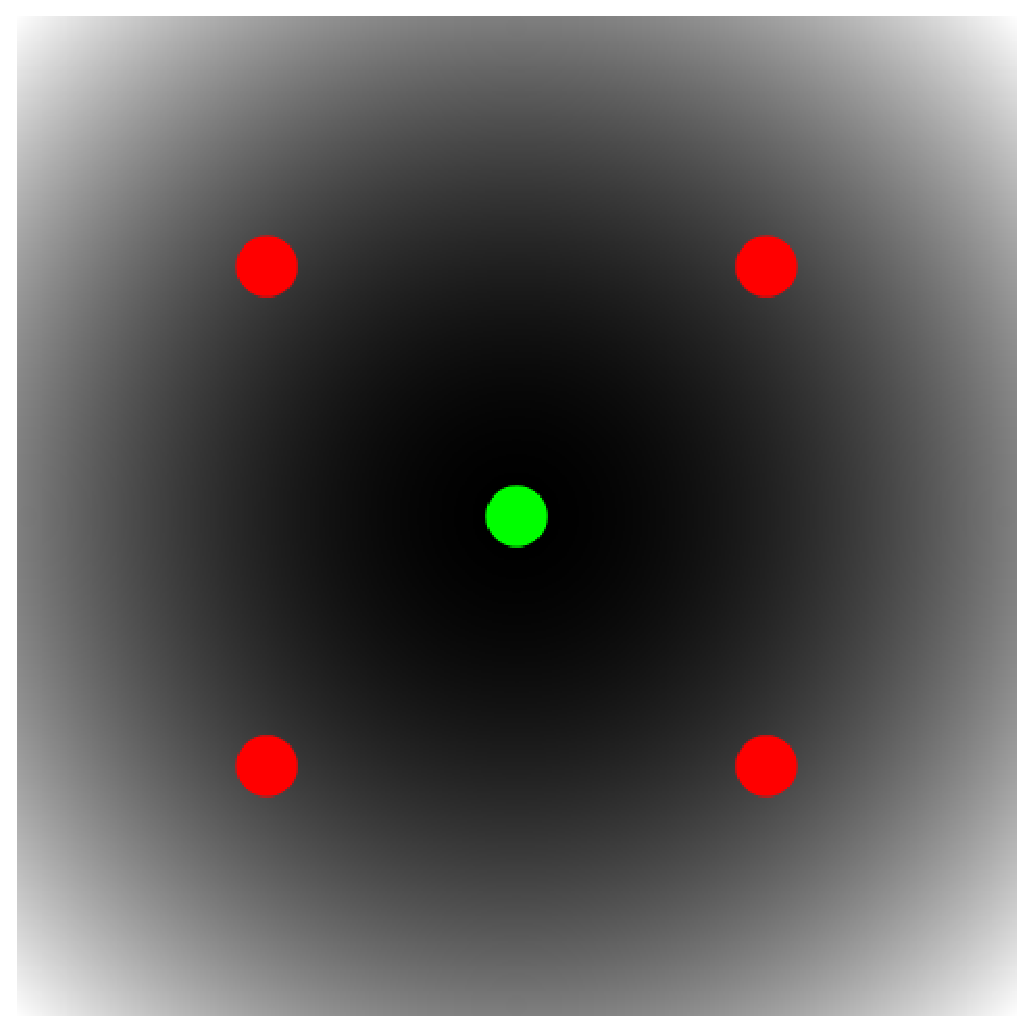
\includegraphics[width=\fwidth]{./figures/spso-0.eps}}&
% 			\onslide<3->\fbox{\includegraphics[width=\fwidth]{./figures/spso-1.eps}}
% 	\end{tabular}
% }
% \end{center}
% \end{example}
% 
% \end{columns}
% 
% \end{frame}
% 
% \subsection{Asynchronous PSO (APSO)}
% 
% \begin{frame}
% \frametitle{Synchronicity in updates}
% \begin{columns}
% \column{.5\textwidth}
% \begin{block}{Asynchronous PSO}
% \begin{algorithm}[H]
% 		\While{not stopping condition}{
% 			\ForEach{\textnormal{Particle} $p \in \mathbb{S}$}{
% 				\color<2,5,8,11>{title.bg}{\textbf<2,5,8,11>{\texttt{p.update();}}}\\
% 				\color<3,6,9,12>{title.bg}{\textbf<3,6,9,12>{\texttt{p.evaluate();}}}\\
% 				\color<4,7,10,13>{title.bg}{\textbf<4,7,10,13>{\texttt{p.communicate();}}}\\
% 			}
% 		}
% \end{algorithm}
% \end{block}
% 
% \column{.5\textwidth}
% \begin{example}
% \begin{center}
% {
% 	\newcommand{\fwidth}{0.4\textwidth}
% 	\setlength\fboxsep{0pt}
% 	\setlength\fboxrule{0.75pt}
% 	\begin{tabular}{cc}
% % 		\onslide<2->$(t)$ & \onslide<5->$(t)$\\
% 			\onslide<2->\fbox{\includegraphics[width=\fwidth]{./figures/apso-0.eps}}&
% 			\onslide<5->\fbox{\includegraphics[width=\fwidth]{./figures/apso-1.eps}}\\
% 			\\
% % 		\onslide<8->$(t)$ & \onslide<11->$(t)$\\
% 			\onslide<8->\fbox{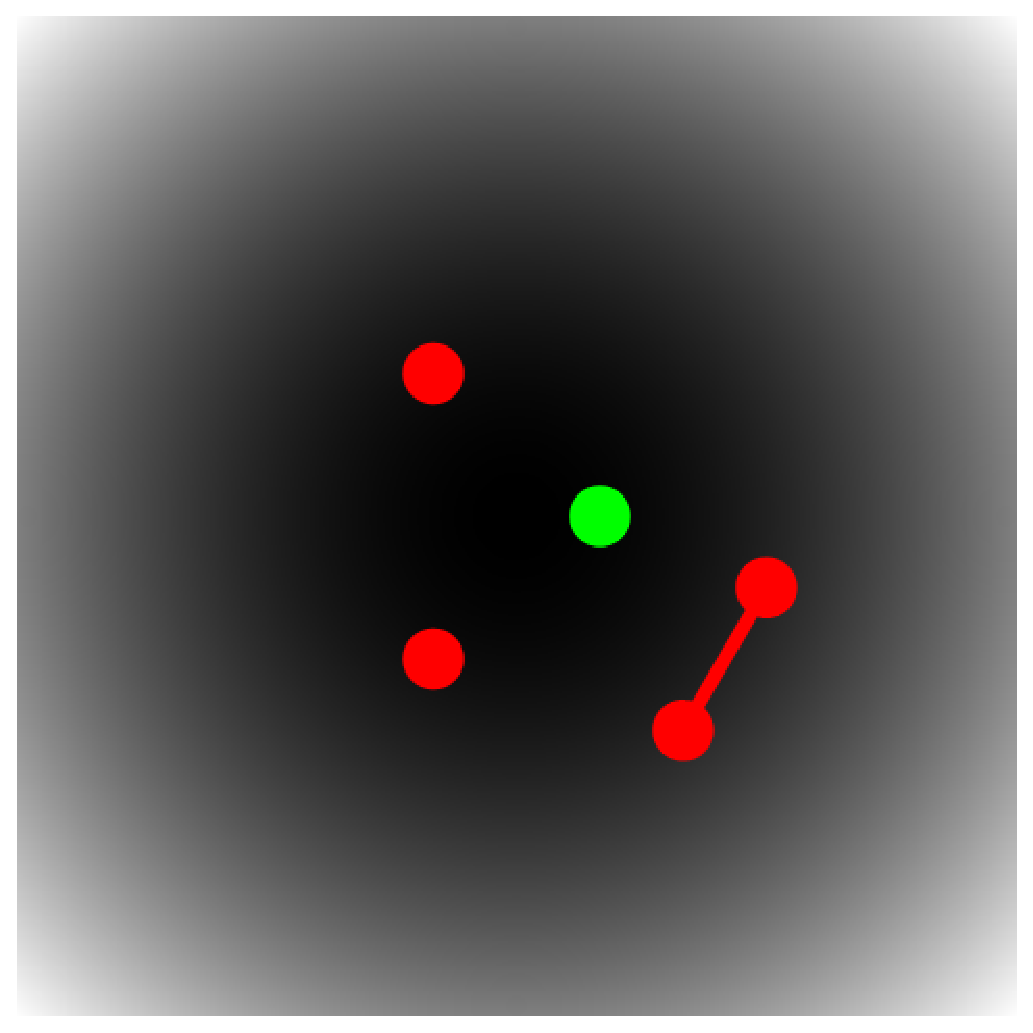
\includegraphics[width=\fwidth]{./figures/apso-2.eps}}&
% 			\onslide<11->\fbox{\includegraphics[width=\fwidth]{./figures/apso-3.eps}}
% 	\end{tabular}
% }
% \end{center}
% \end{example}
% 
% \end{columns}
% \end{frame}
% 
% 
% 
% 
% 
% \section{Experimental Design}
% \subsection{Benchmark functions}
% 
% \begin{frame}
% \frametitle{Experimental Design}
% 
% \begin{columns}
% \column{.5\textwidth}
% \vspace{-10pt}
% \begin{block}{Benchmark functions}<1->
% \newcommand{\fwidth}{0.15\textwidth}
% \setlength\fboxsep{0pt}
% \setlength\fboxrule{0.75pt}
% 
% \setlength{\tabcolsep}{2pt}
% \footnotesize
% \renewcommand\arraystretch{0.8}
% 
% \begin{tabular}{rccl}
% 	\multicolumn{2}{c}{\textbf{Unimodal}} &
% 	\multicolumn{2}{c}{\textbf{Multimodal}}\\
% 	\hline\\
% 	&\multirow{3}{*}{\fbox{
\includegraphics[width=\fwidth]{./figures/quadric.eps}}}
% 	& \multirow{3}{*}{\fbox{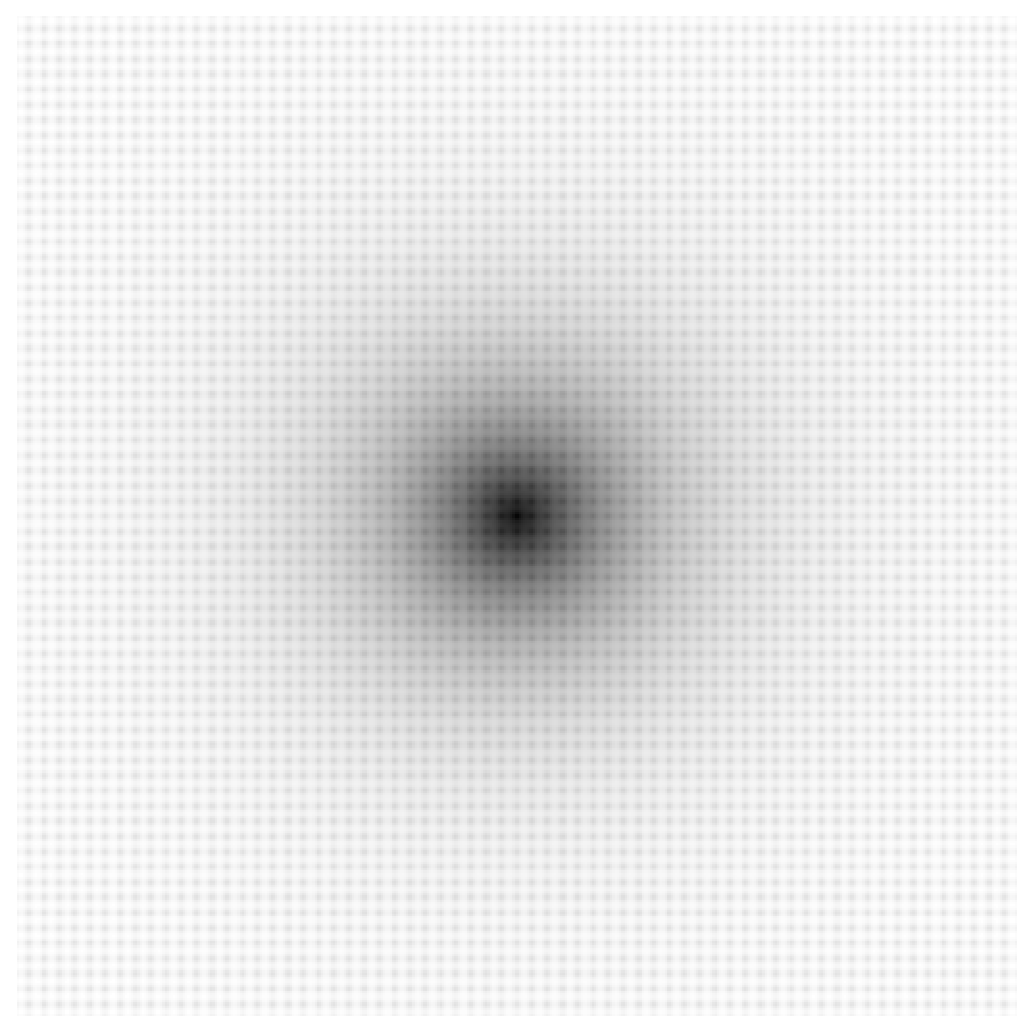
\includegraphics[width=\fwidth]{./figures/ackley.eps}}} \\
% 	Quadric &&& Ackley\\
% 	\\
% 	
% 	 &\multirow{3}{*}{\fbox{
\includegraphics[width=\fwidth]{./figures/quartic.eps}}}
% 	 &
% 	 \multirow{3}{*}{\fbox{
\includegraphics[width=\fwidth]{./figures/griewank.eps}}}\\
% 	 Quartic &&& Griewank\\
% 	 \\
% 	
% 	&\multirow{3}{*}{\fbox{
\includegraphics[width=\fwidth]{./figures/rosenbrock.eps}}}
% 	&
% 	\multirow{3}{*}{\fbox{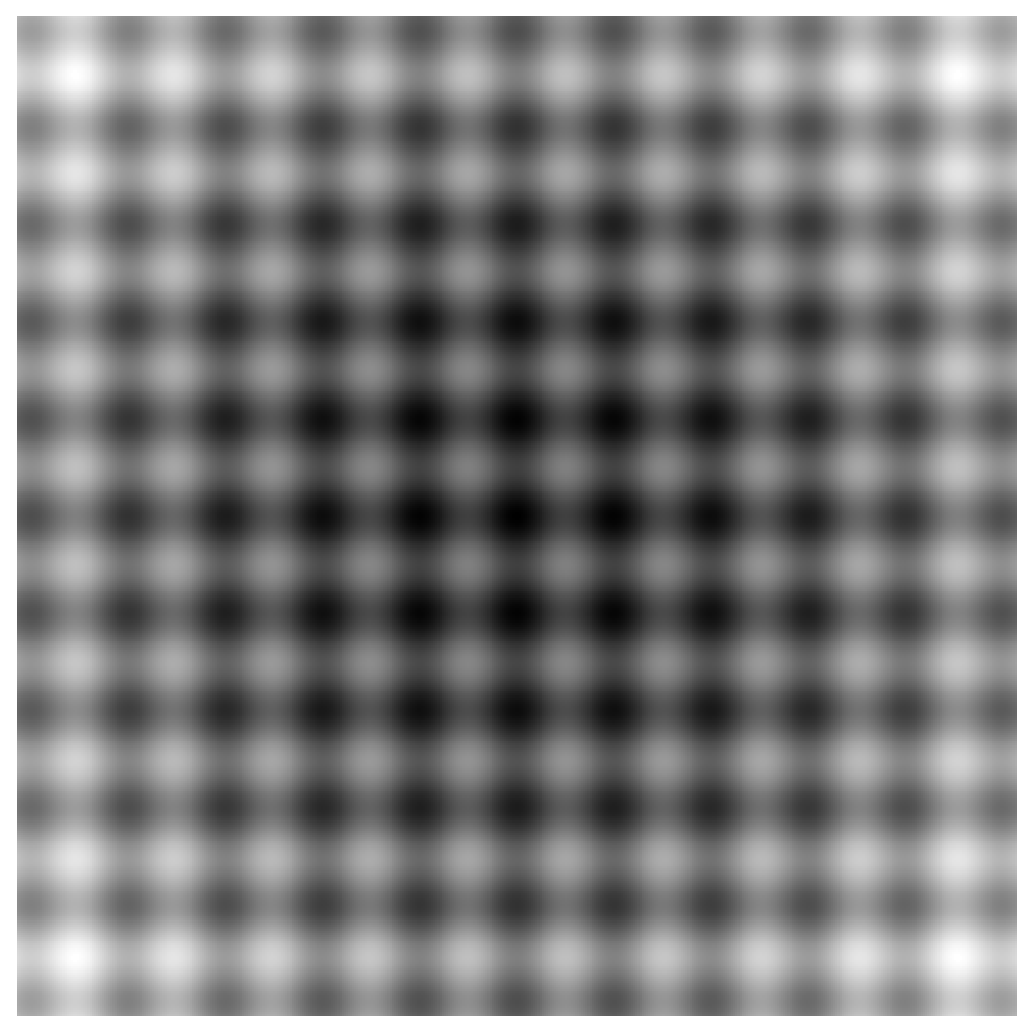
\includegraphics[width=\fwidth]{./figures/rastrigin.eps}}}\\
% 	\alert<2>{Rosenbrock} &&& Rastrigin\\
% 	\\
% 	
% 	&\multirow{3}{*}{\fbox{
\includegraphics[width=\fwidth]{./figures/spherical.eps}}}
% 	&\multirow{3}{*}{\fbox{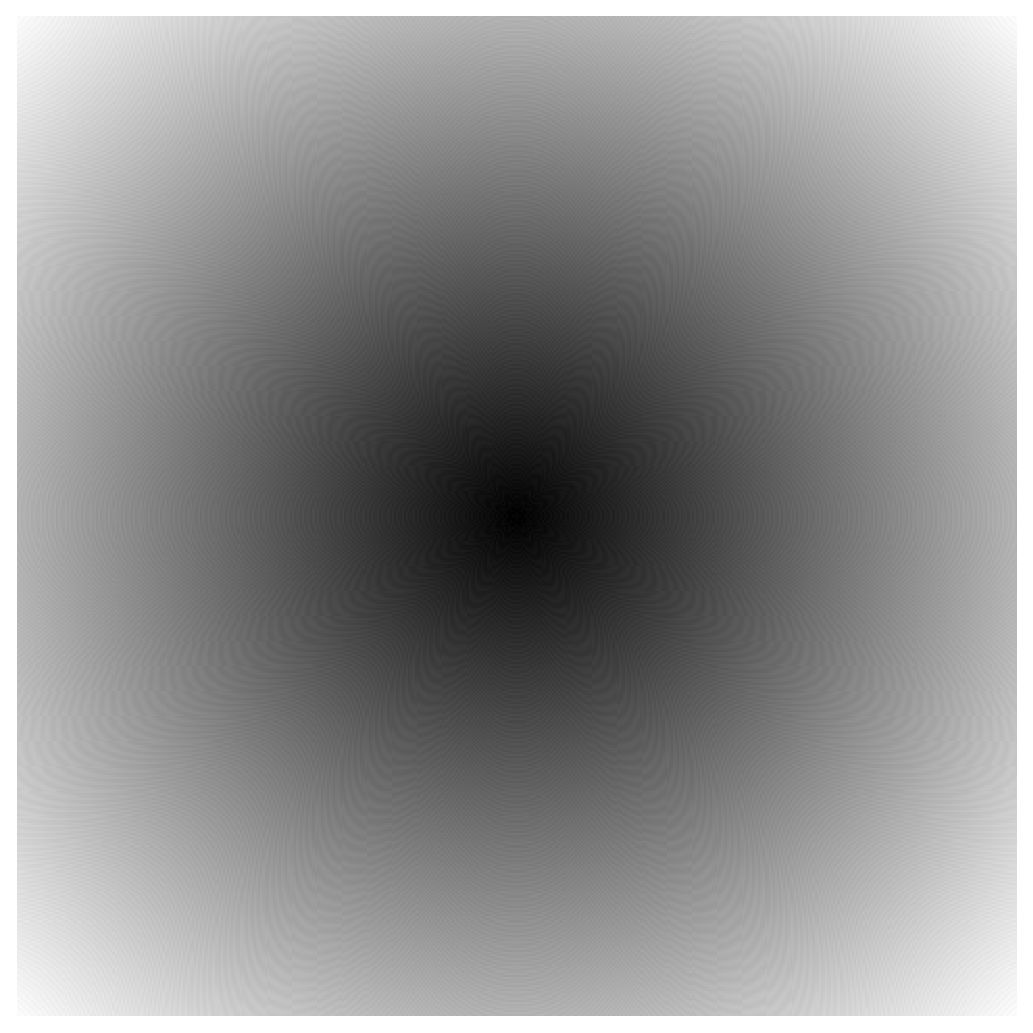
\includegraphics[width=\fwidth]{./figures/salomon.eps}}}\\
% 	Spherical &&& Salomon\\
% 	\\
% 	
% 	&\multirow{3}{*}{\fbox{
\includegraphics[width=\fwidth]{./figures/hyperellipsoid.eps}}}
% 	&\multirow{3}{*}{\fbox{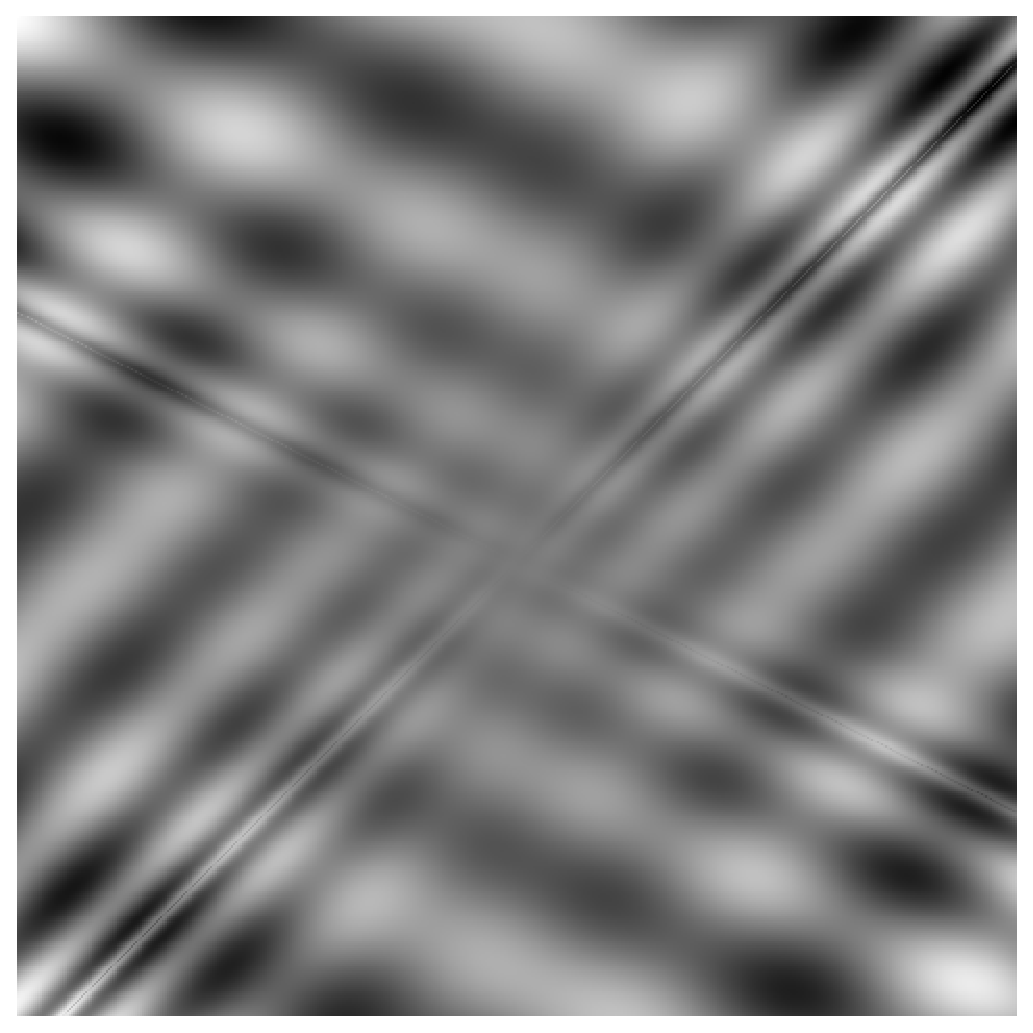
\includegraphics[width=\fwidth]{./figures/eggholder.eps}}}\\
% 	HyperEllipsoid &&& EggHolder\\
% 	\\
% 	
% \end{tabular}
% \end{block}
% 
% 
% \column{.5\textwidth}
% \vspace{-10pt}
% \begin{block}{Parameters}<3->
% {
% 
% \begin{itemize}
%   \setlength\itemindent{-1em}
%   \item<3-> 50 Runs, 300 Iterations
%   
%   \setlength\itemindent{-1em}
%   \item<4-> 30 particles in $\mathbb{R}^{30}$
%   
%   \setlength\itemindent{-1em}
%   \item<5-> Neighbors: $n=\{2,6,14,22,30\}$
%  
%   \setlength\itemindent{-1em}
%   \item<6-> Acceleration: $c_1=c_2=1.49618$
%   
%   \setlength\itemindent{-1em}
%   \item<6-> Inertia: $w=0.729844$
%   
%   \setlength\itemindent{-1em}
%   \item<6-> Velocity clamping: $\tanh$
%   
%   \setlength\itemindent{-1em}
%   \item<6-> $V_{\max} = \frac{1}{4} \cdot \left|x_{\max} - x_{\min}\right|$
% \end{itemize}
% }
% \end{block}
% 
% 
% \end{columns}
% 
% \vspace{5pt}
% \begin{columns}
% \column{0.05\textwidth}
% \column{0.9\textwidth}
% \vspace{-10pt}	
% \begin{block}{Performance indicators}<7->
% \vspace{-10pt}
% \begin{columns}
% 	\column{0.5\textwidth}
% 	\begin{itemize}
% 	  \item Quality of results
% 	\end{itemize}
% 	\column{0.5\textwidth}
% 	\begin{itemize}
% 	  \item Speed of convergence
% 	\end{itemize}
% \end{columns}
% \end{block}
% \column{0.05\textwidth}
% \end{columns}
% \end{frame}
% 
% 
% \subsection{Performance indicators}
% 
% \begin{frame}
% \frametitle{Performance indicators}
% 
% \begin{block}{Quality of results}
% % 	\begin{itemize}
% % 	  \item Minimization problems
% % 	\end{itemize}
% 	\begin{figure}
% 		\includegraphics[width=0.95\textwidth]{./figures/quality-example.eps}
% 	\end{figure}
% \end{block}
% \end{frame}
% 
% 
% \begin{frame}
% \frametitle{Performance indicators}
% \begin{columns}
% \column{0.5\textwidth}
% \begin{block}{Speed of convergence}<1->
% \begin{itemize}
%   \item Which one is \textbf{\emph{faster}}?
% \end{itemize}
% 	\begin{figure}
% 		\includegraphics[width=\textwidth]{./figures/speed-of-convergence.eps}
% 	\end{figure}
% \end{block}
% 
% \column{0.5\textwidth}
% \begin{block}{Multi-objective problem}<2->
% \begin{itemize}
%   \item Area Under the Curve ($I_H$)
% \end{itemize}
% \begin{figure}
% 	\includegraphics[width=\textwidth]{./figures/auc-example.eps}
% \end{figure}
% \note{The smallest the better}
% \end{block}
% \end{columns}
% \end{frame}
% 
% 
% 
% 
% \section{Results and Discussion}
% \subsection{Unimodal functions}
% % \subsubsection{Unimodal functions}
% \begin{frame}
% \frametitle{Unimodal functions}
% 
% \begin{block}{Quality of results}
% 	\begin{figure}
% 		\includegraphics[width=0.5\textwidth]{./figures/quality-quartic.eps}
% 		\includegraphics[width=0.5\textwidth]{./figures/quality-spherical.eps}
% 	\end{figure}
% \end{block}
% 
% \begin{columns}
% 	\column{0.075\textwidth}
% 	\column{0.25\textwidth}
% 	\begin{block}{}
% 	\begin{figure}
% 		\includegraphics[width=\textwidth]{./figures/quality-example-miniature.eps}
% 	\end{figure}
% 	\end{block}
% 	
% 	\column{0.6\textwidth}
% % \begingroup
% % \setbeamercolor{block title}{fg=black,bg=gray!40}
% % \setbeamercolor{block body}{fg=black,bg=gray!10}
% % \setbeamercolor{itemize item}{fg=gray} % all frames will have red bullets
% % \setbeamerfont{block title}{series=\bfseries}
% 	\begin{block}{}
% 	\centering
% 		\begin{itemize}
% 		  \setlength\itemindent{-1em}
% 		  \item Neighbors:\\
% 		  \setlength\parindent{-1em}
% 		  $\{a=2,\; b=6,\; c=14,\; d=22,\;e=30\}$
% 		  \setlength\itemindent{-1em}
% 		  \item {\color{block title example.bg}SPSO} and {\color{red}APSO$^*$} 
% 		\end{itemize}
% 	\end{block}
% 	\column{0.075\textwidth}
% % \endgroup
% % 	\column{0.05\textwidth}
% \end{columns}
% 
% \end{frame}
% 
% 
% \begin{frame}
% \frametitle{Unimodal functions}
% 
% \begin{block}{Speed of convergence}
% 	\begin{figure}
% 		\includegraphics[width=0.5\textwidth]{./figures/auc-quartic.eps}
% 		\includegraphics[width=0.5\textwidth]{./figures/auc-spherical.eps}
% 	\end{figure}
% \end{block}
% 
% \begin{columns}
% 	\column{0.075\textwidth}
% 	\column{0.25\textwidth}
% 	\begin{block}{}
% 	\begin{figure}
% 		\includegraphics[width=\textwidth]{./figures/quality-example-miniature.eps}
% 	\end{figure}
% 	\end{block}
% 	
% 	\column{0.6\textwidth}
% % \begingroup
% % \setbeamercolor{block title}{fg=black,bg=gray!40}
% % \setbeamercolor{block body}{fg=black,bg=gray!10}
% % \setbeamercolor{itemize item}{fg=gray} % all frames will have red bullets
% % \setbeamerfont{block title}{series=\bfseries}
% 	\begin{block}{}
% 	\centering
% 		\begin{itemize}
% 		  \setlength\itemindent{-1em}
% 		  \item Neighbors:\\
% 		  \setlength\parindent{-1em}
% 		  $\{a=2,\; b=6,\; c=14,\; d=22,\;e=30\}$
% 		  \setlength\itemindent{-1em}
% 		  \item {\color{block title example.bg}SPSO} and {\color{red}APSO$^*$} 
% 		\end{itemize}
% 	\end{block}
% 	\column{0.075\textwidth}
% % \endgroup
% % 	\column{0.05\textwidth}
% \end{columns}
% 
% \end{frame}
% 
% 
% \subsection{Multimodal functions}
% \begin{frame}
% \frametitle{Multimodal functions}
% 
% \begin{block}{Quality of results}
% 	\begin{figure}
% 		\includegraphics[width=0.5\textwidth]{./figures/quality-rastrigin.eps}
% 		\includegraphics[width=0.5\textwidth]{./figures/quality-griewank.eps}
% 	\end{figure}
% \end{block}
% 
% \begin{columns}
% 	\column{0.075\textwidth}
% 	\column{0.25\textwidth}
% 	\begin{block}{}
% 	\begin{figure}
% 		\includegraphics[width=\textwidth]{./figures/quality-example-miniature.eps}
% 	\end{figure}
% 	\end{block}
% 	
% 	\column{0.6\textwidth}
% % \begingroup
% % \setbeamercolor{block title}{fg=black,bg=gray!40}
% % \setbeamercolor{block body}{fg=black,bg=gray!10}
% % \setbeamercolor{itemize item}{fg=gray} % all frames will have red bullets
% % \setbeamerfont{block title}{series=\bfseries}
% 	\begin{block}{}
% 	\centering
% 		\begin{itemize}
% 		  \setlength\itemindent{-1em}
% 		  \item Neighbors:\\
% 		  \setlength\parindent{-1em}
% 		  $\{a=2,\; b=6,\; c=14,\; d=22,\;e=30\}$
% 		  \setlength\itemindent{-1em}
% 		  \item {\color{block title example.bg}SPSO} and {\color{red}APSO$^*$} 
% 		\end{itemize}
% 	\end{block}
% 	\column{0.075\textwidth}
% % \endgroup
% % 	\column{0.05\textwidth}
% \end{columns}
% 
% \end{frame}
% 
% 
% 
% \begin{frame}
% \frametitle{Multimodal functions}
% 
% \begin{block}{Speed of convergence}
% 	\begin{figure}
% 		\includegraphics[width=0.5\textwidth]{./figures/auc-rastrigin.eps}
% 		\includegraphics[width=0.5\textwidth]{./figures/auc-griewank.eps}
% 	\end{figure}
% \end{block}
% 
% \begin{columns}
% 	\column{0.075\textwidth}
% 	\column{0.25\textwidth}
% 	\begin{block}{}
% 	\begin{figure}
% 		\includegraphics[width=\textwidth]{./figures/quality-example-miniature.eps}
% 	\end{figure}
% 	\end{block}
% 	
% 	\column{0.6\textwidth}
% % \begingroup
% % \setbeamercolor{block title}{fg=black,bg=gray!40}
% % \setbeamercolor{block body}{fg=black,bg=gray!10}
% % \setbeamercolor{itemize item}{fg=gray} % all frames will have red bullets
% % \setbeamerfont{block title}{series=\bfseries}
% 	\begin{block}{}
% 	\centering
% 		\begin{itemize}
% 		  \setlength\itemindent{-1em}
% 		  \item Neighbors:\\
% 		  \setlength\parindent{-1em}
% 		  $\{a=2,\; b=6,\; c=14,\; d=22,\;e=30\}$
% 		  \setlength\itemindent{-1em}
% 		  \item {\color{block title example.bg}SPSO} and {\color{red}APSO$^*$} 
% 		\end{itemize}
% 	\end{block}
% 	\column{0.075\textwidth}
% % \endgroup
% % 	\column{0.05\textwidth}
% \end{columns}
% 
% \end{frame}
% 
% 
% 
% \section{Conclusions and Future Work}
% 
% \subsection*{Conclusions}
% \begin{frame}
% \frametitle{Conclusions}
% 	\begin{block}{}
% 	\vspace{6pt}
% 	\begin{itemize}[<+->]
% 	  \setlength{\itemsep}{6pt}
% 	  \item SPSO is better and similar (or even faster) than APSO
% 	  \item Unimodal: larger neighborhoods favors quality and speed
%  	  \item Multimodal: 
% 	  \begin{itemize}
% 	  \item SPSO: larger neighborhoods favor speed but not much quality
% 	  \item APSO: same as SPSO, but gap in quality and speed is closer
% 	  \end{itemize}
% 
% 	  \item Speed of convergence as a multi-objective problem
% 	  \item Importance of robust statistics and statistical tests
% 	\end{itemize}
% 	\vspace{1pt}
% 	\end{block}
% 
% \end{frame}
% 
% 
% \subsection*{Future Work}
% \begin{frame}
% \frametitle{Future Work}
% 
% \begin{block}{}
% 	\vspace{10pt}
% 	\begin{itemize}[<+->]
% 	  \setlength{\itemsep}{10pt}
% 	  \item Compare SPSO and APSO on other benchmark functions
% 	  \item Especially on benchmark functions of greater complexity
% 	  \item Experiment with different parameters
% 	  \item Explore different multi-objective performance indicators
% 	\end{itemize}
% 	\vspace{10pt}
% \end{block}
% 
% \end{frame}
% 
% 
% % \section*{Appendix}
% % \begin{frame}
% % \frametitle{Equations}
% % % \begin{block}{Equations}
% % % 	
% % % \begin{equation}
% % % 	\begin{split}
% % % 		x_i(t+1) =& x_i(t) + v_i(t+1)\\
% % %   		v_i(t+1) =& wv_i(t) + c_1r_1(t)[y_i(t) - x_i(t)]\\
% % %   				  & + c_2r_2(t)[\hat{y}_i(t) - x_i(t)]
% % % 	\end{split}
% % % \end{equation}
% % % 	
% % % \end{block}
% % \end{frame}
% % 
% % \begin{frame}
% % \frametitle{More results}
% % \end{frame}
% 
% 
% 
% % \section{Particle Swarm Optimization}
% % 
% % \begin{frame}
% % \frametitle{}
% % 
% % \begin{definition}
% % 	$x(t + 1) = x(t) + v(t+1)$\\
% % 	$v(t + 1) = wv(t) + c_1r_1(y - x) +  c2_r2(y - x)$
% % \end{definition}
% % 
% % \begin{block}{Some block}
% % 	This is a block;
% % \end{block}
% % 
% % \begin{columns}
% % \column{.5\textwidth}
% % \begin{block}{Answered Questions}
% % How many primes are there?\cite{Goldbach1742}
% % 
% % \end{block}
% % \column{.5\textwidth}
% % \begin{block}{Open Questions}
% % Is every even number the sum of two primes?
% % \end{block}
% % \end{columns}
% % 
% % 
% % 
% % 
% % % You can create overlays
% % \begin{itemize}
% %   \item using the \texttt{pause} command:
% %   \begin{itemize}
% %     \item First item.
% %     \pause
% %     \item Second item.
% %   \end{itemize}
% %   \item using overlay specifications:
% %   \begin{itemize}
% %     \item<3-> First item.
% %     \item<4-> Second item.
% %   \end{itemize}
% %   \item using the general \texttt{uncover} command:
% %   \begin{itemize}
% %     \uncover<5->{\item First item.}
% %     \uncover<6->{\item Second item.}
% %   \end{itemize}
% % \end{itemize}
% % \end{frame}
% % 
% % \section*{Summary}
% % 
% % 
% % 
% % \begin{frame}
% % \frametitle<presentation>{Summary}
% % 
% % \begin{itemize}
% %   \item The \alert{first main message} of your talk in one or two lines.
% % \end{itemize}
% % 
% % % The following outlook is optional.
% % \vskip0pt plus.5fill
% % \begin{itemize}
% %   \item Outlook
% %   \begin{itemize}
% %     \item Something you haven't solved.
% %     \item Something else you haven't solved.
% %   \end{itemize}
% % \end{itemize}
% % \end{frame}
% % 
% % \begin{thebibliography}{10}
% % \bibitem{Goldbach1742}[Goldbach, 1742]
% % Christian Goldbach.
% % \newblock A problem we should try to solve before the ISPN ’43 deadline,
% % \newblock \emph{Letter to Leonhard Euler}, 1742.
% % \end{thebibliography}
% 

\end{document}
